\documentclass{article}

\usepackage[utf8]{inputenc}
\usepackage[]{algorithm2e}
\usepackage{graphicx}
\usepackage{amsmath}
\graphicspath{ {images/} }
\usepackage{svg}
\usepackage[letterpaper, portrait, margin=1in]{geometry}
\usepackage{multicol}
\setlength{\columnsep}{1cm}
\usepackage[english]{babel}
\usepackage{csquotes}
\usepackage{mfirstuc}
\usepackage[
  backend=biber,
  style=authoryear-icomp,
  url=true
]{biblatex}
\addbibresource{whitepaper.bib}

%% \addtocontents{toc}{\protect\setcounter{tocdepth}{0}}

\newcommand{\mesh}{Orchid}
\newcommand{\Mesh}{\mesh}

\usepackage{titlesec}
\titlelabel{\thetitle.\quad}

\title{\mesh{}: A Fully Distributed, Anonymous Proxy Network Incentivized Through Bandwidth Mining}
%%\title{\mesh{}: Micropayment Networking}
\author{{David L. Salamon with} \\ {Brian J. Fox, Jay Freeman, Gustav Simonsson,} \\ {{Stephen F. Bell, and Dr. Steven Waterhouse, Ph.D.}}}
\date{September 19, 2017}

\raggedbottom

\begin{document}

\maketitle

\begin{abstract}

  As methods for censoring browsing and discovering private browsing information have improved, interest in anonymization methods has increased. Unfortunately, existing approaches to unrestricted, unsurveilled Internet access such
as I2P and Tor suffer from a tragedy of the commons – only a few thousand unpaid volunteers host proxies and exit nodes, allowing sophisticated attackers a tractable number of nodes to monitor or otherwise compromise. We present a market based, fully decentralized, anonymous peer-to-peer system based on “bandwidth mining” which we hope will address this lack of relays by paying them.

  %% The Internet's current structure is the product of two forces: (1)
  %% what is easy to implement for a small to medium sized company, and
  %% (2) the desires of mankind.

  %% Unfortunately, not all desires of mankind have proved agreeable. For
  %% example, as methods for censoring browsing and discovering private
  %% browsing information have improved, consumers have found themselves
  %% in the unenviable position of needing to decide between their
  %% privacy and usable Internet access. Even for those willing to suffer
  %% the usability hit, current methods to achieve unrestricted,
  %% unsurveilled Internet access such as I2P and Tor suffer from a
  %% tragedy of the commons – only a few thousand unpaid volunteers host
  %% proxies and exit nodes, allowing sophisticated attackers a tractable
  %% number of nodes to monitor or otherwise compromise.

  %% Similarly, not all desirable services have proved easy to
  %% implement. Perverse economic incentives stemming from widely
  %% available free content have resulted in a news media bereft of
  %% subscribers, slowly descending into a minute-to-minute battle for
  %% clicks. The high cost of distributing video has resulted in
  %% centralization, platforms, and burdens on content creators. The
  %% difficulty of maintaining and securing a sever have resulted in less
  %% diversity than one might have hoped for.

  %% To address these issues, we present a high performance approach to
  %% networking built on a foundation of micropayments, and as an initial
  %% application of the technology, build an uncensorable, anonymous
  %% mechanism for accessing the global Internet. It is our hope that as
  %% the tokens gain in acceptance, many millions of websites will
  %% incorporate the payment models described here, and consumers will
  %% receive a monthly budget of tokens from their ISP.

  Contributions include:

  \begin{itemize}
  \item A payment mechanism suitable for transactions as inexpensive
    as a ten-thousandth of a penny, up to arbitrarily high
    denominations.
  \item A commodity specification for the sale of bandwidth.
  \item A method for distributed inductive proofs in peer-to-peer
    systems which make Eclipse attacks arbitrarily difficult.
  \item An efficient security-hardened auction mechanism suited for
    the sale of bandwidth in circumstances where an attacker may alter
    their bid as part of an attack.
  \item A fully distributed anonymous bandwidth market.
  \end{itemize}

\end{abstract}


\newpage
\tableofcontents
\newpage


\section{Introduction}
\label{sec:overview}

\subsection{System Goals}

The \mesh{} Network was designed with three goals:

\begin{enumerate}
\item To codify the right to unrestricted, unsurveilled Internet access on a networking level.
\item To build a system suited for daily use. To say that a freedom is not a part of daily life is to say that the freedom is dying.
\item To make such a system worthy of trust, by developing it in the open and releasing the source code for full public audit.
\end{enumerate}

These are ambitious goals, and are not realized by the system described in this document. This document does, however, contain an imperfect first attempt – an invitation to join us in design, construction, and use of what we believe is the future of networking.

\subsection{Acknowledgements}

Professor Boneh, Professor Vigna, Justin Sheek. Add people!

\subsection{Document Structure}

This document begins with an overview of the system (Section \ref{sec:overview}), describes the kind of attacks and attackers that can be reasonably anticipated against such a system (Section \ref{sec:attacks}), and then discusses the lessons that can be learned from the previous deployment of similar systems (Section \ref{sec:prior-work}). We include these sections in the hope that they might help jog the readers memory, perhaps alert them to interesting references, and assist intuition for the context in which the system will be deployed.

Once the stage has been set, we will move on to a detailed discussion of the system components themselves. We will detail the external libraries we have chosen to rely on, and why (Section \ref{sec:external-libraries}), describe a micropayment system suited to the sale of bandwidth (Section \ref{sec:tickets}), a commodity specification for the sale of bandwidth (Section \ref{sec:mining}), a distributed marketplace for the sale of bandwidth (Section \ref{sec:agora}), and a method of employing our commodity specification for bandwidth to build an uncensorable and anonymously Internet connection (Section 8). This is to say these sections provide a “nuts and bolts” view of the Agora network. Each component uses the previous as building blocks, so it is recommended that you read these sections in order.

We close out with a discussion of what an attacker's experience of the system might be (Section \ref{sec:attack-stories}), both as a means of discussing the security of the system when viewed as a whole, and as a thought experiments for those wishing to assist us in improving system security. Next we discuss non-security features we hope to add in future releases (Section \ref{sec:future}). Readers interested in assisting with the project are encouraged to read these sections carefully.

Because the system is to be fully decentralized, fully autonomous, and fully anonymous, much of this design document is centered on attacks. Although attack analysis is important, and will take up much of our time, it is ultimately no more than a necessary conceit to the context in which the market is to operate; please do not let thoughts of security distract you unduly from an understanding the system itself. We look forward to conversing about the system with experts in economics, autonomous markets, network engineers, applications programmers, and anyone with interest.

\subsection{Terms}

\begin{itemize}
\item Node. A computer running a program which implements the \mesh{} Protocol.
\item Medallion. Data used by a node to demonstrate it is in exclusive possession of computational resources.
\item User. The owner of a node.
\item Agora. A collection of nodes interacting through the \mesh{} Distributed Marketplace Protocol.
\item \emph{The} Agora. The Agora in possesion of the most global computational power.
\item Econ. A node who is a member of an Agora's collection.
\item Entry Econ. An econ who is willing to accept direct TCP connections from Users.
\item Address. The location in Medallion-space inhabited by an Econ.
\item Customer. A buyer on the Agora.
\item Relay. A node willing to sell bandwidth to customers.
\item Proxy. A relay which is additionally willing to interact with web servers on behalf of customers.
\item Manifold. A chain of relays used for anonymous communication.
\item Ticket. A stochastic micropayment.
\item Attack. A method for causing the non-consensual transfer of money or information.
\item Attacker. A person or group of people interested in performing attacks.
\end{itemize}

\subsection{Core Security Assumptions}
\label{core-security}

The security of the \mesh{} system as a whole ultimately rests on basic assumptions about the world. In the event this assumption is ever falsified, the system will not function as intended.

\begin{itemize}
\item The majority of global computation power will not cooperate on an attack.
\end{itemize}

Without this assumption (or a similar for a different resource), it would be impossible for a fully anonymous and distributed system to function. No distributed quorum could be trusted, because the majority of users might vote in such a way as to facilitate attacks. Users would be left relying on web-of-trust approaches, which by their nature are non-anonymous.

We use this assumption, combined with a method for rapidly demonstrating significant computational work has been done, to construct the basis for trust on our system: medallions. Production of a medallion ties ownership of computation to a public key. They are presented as needed to prove that a given node is “real.” For a more detailed discussion see Section \ref{medallion}.

\subsection{High-Level System Overview}

\subsubsection{The Agora}

\begin{figure}[htbp]
  \centering
  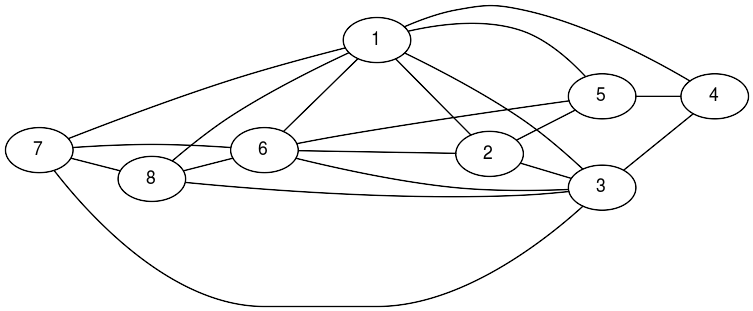
\includegraphics[width = 300pt]{agoraOverview}
  \caption{An Agora with eight Econs}
\end{figure}

The Agora is a globally distributed P2P market place for bandwidth. Although it is tempting to believe such a market should take the form of a classic order book (a list of currently unfilled bids and asks at different prices), a very important property of bandwidth to be used for anonymity purposes is that purchase decisions are made in a way that places severe limits on what influence can be exerted by an attacker. For this reason, rather than provide an order book, the Agora provides a way to traverse the space of currently valid medallions. Once a location in medallion-space has been selected, a miniature pseudo-auction is held. For example, if the econ at position 2 in the figure wished to buy bandwidth, it would select the median of 1’s, 3’s, 5’s and 6’s price, rounded down. For users not seeking anonymity, the lowest price may be selected instead.

\subsubsection{Manifolds}

\begin{figure}[htbp]
  \centering
  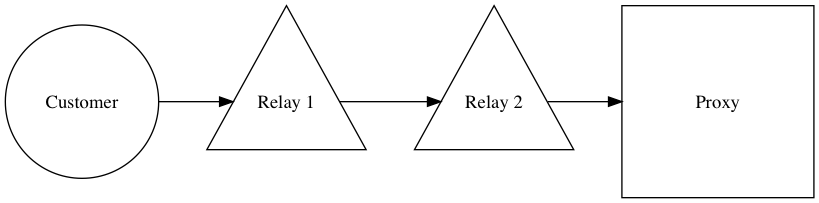
\includegraphics[width = 300pt]{sttc}
  \caption{A three-Econ Manifold routing traffic for a Customer}
\end{figure}

Once relay and proxy bandwidth has been purchased, the customer configures them into a connected chain termed a manifold. In the above picture, Relay 1 receives bandwidth from the Customer, performs cryptographic operations on it, and forwards it to Relay 2. Relay 2 performs a similar role with respect to Relay 1 and the Proxy. The Proxy then sends this data to a web server. Any data returned by the web server is sent back to the Customer along another manifold, perhaps implemented using the same nodes in reverse.

\subsubsection{Web Browsing}

The majority of initial usage of the \mesh{} Network will likely happen in support of uncensorable, anonymous web browsing. In this use case, the client software will automatically use the Agora to create a manifold, and provide additional checks to verify that SSL/TLS is being used in a way suited to this networking model. Unless two or more nodes in a manifold are working together (Section \ref{sec:collusion}), perhaps because they are run by the same user, no single node knows the Customer's IP Address and the server they communicated with.

\subsection{User Stories}

\subsubsection{Bandwidth Miners}

Users with excess computational power and bandwidth may choose to support the \mesh{} project, as well as earn money, by running an econ on their computer. To do so, they install and run the \mesh{} software package and supply a payment address. To verify realness while preserving anonymity, the software will convert computational resources into Medallions. Econs are compensated for their lost computation by bandwidth customers.

\subsubsection{Resisting Oppressive Governments}

Users who live under oppressive regimes (where, for example, it is illegal to access Wikipedia), can use the system to hide information about the websites they are browsing. To do so they install and run the \mesh{} software, provide an initial payment to their \mesh{} wallet, and browse the web as normal. Unlike similar services (Section \ref{sec:prior-work}), the network pays hosts for their participation. We hope this will lead to greater participation, which in turn will lead to grater anonymity (Section \ref{sec:agora}).

\subsubsection{Resisting Oppressive Web Applications}

Users of oppressive web applications (sites which change services offered based on geographic location), can use the \mesh{} Network to appear to be browsing from the country of their choice. Unlike similar services (Section \ref{sec:prior-work}), traffic will not come from IP ranges allocated to server farms, and so will be much harder for oppressive websites to block. Additionally, because bandwidth is incentivized, it will likely prove much more plentiful on the \mesh{} Network, i.e. making the real-time playback of high resolution video viable.


\section{Attacks}
\label{sec:attacks}

\subsection{Bug Bounty / White Hat Policy}

TODO: we should offer a “hall of fame”, a cash/token reward, and maybe a t-shirt or coffee mug or something?

Note that token rewards are very interesting, since we could set aside a fixed amount and pay out x\% of that amount for each vulnerability which is found.. it would likely become the largest bug bounty program in history. If the issue is that putting those tokens aside might be difficult at this point, I also think that incentivizing vulnerability disclosure this a very compelling reason to inflate the currency.

\subsection{Attacker Goals}

\subsubsection{Information Gathering}

The largest class of attacks against which the \mesh{} Protocol must defend against are those which reveal information about its users. Because \mesh{} is implemented as an overlay on the existing Internet, some information is unavoidably shared with some peers. In the list below, such information is marked with a “*”. Any information which is not specifically listed as unavoidably shared in this document, but for which a method is discovered to uncover that information is termed an \emph{informational attack} and is covered by \mesh{}’s White Hat Bug Bounty. For more information on what is shared, see the protocol specification in Section \ref{sec:mining} and discussion of collusion in Sction \ref{sec:collusion}, and our reference implementation of the network \cite{oursoftware}.

Types of data which are assumed to be of interest to an attacker (timeless):

\begin{itemize}
\item Real-World Identity Information. A user’s given name, SSN, address, etc.
\item Website Account Information. The user accounts at a specific website. Note this can be different from Real-World Identity Information.
\item *IP Information. The IP address from which a user is accessing the \mesh{} Network. Note that in some usage scenarios this may be equivalent to learning Real-World Identity Information.
\item *Ethereum Information. The keys associated with a user’s wallet (*public or private). Note that in some usage scenarios this may be equivalent to learning Real-World Identity Information.
\item *\mesh{} Network Information. The keys associated with a node’s current business on the \mesh{} network (*public or private).
\end{itemize}

Types of Behavioral information which are assumed to be of interest to an attacker (time and manifold associated data):

\begin{itemize}
\item *Customer Identification. The attacker learns the IP address of a customer.
\item *Relay Identification. The attacker learns the IP address of a relay.
\item *Proxy Identification. The attacker learns the IP address of a proxy.
\item *Link Identification. The attacker learns that two IP addresses where employed in a manifold.
\item *Website Access. The attacker learns that an outbound connection was made from the \mesh{} network to a specific website.
\item *Webserver Access. The attacker learns that an outbound connection was made from the \mesh{} network to a specific webserver (which may host multiple websites).
\item *Ethereum Linking. The attacker learns that an Ethereum public key is held by a \mesh{} user.
\item *Purchase Linking. The attacker learns that two transactions share a common payer.
\item *Purchase Information. The attacker learns the quantity and timing of bandwidth sent over a Manifold.
\end{itemize}

Although all of the above behavioral information is shared with other nodes on the \mesh{} Network during normal operation, as described below, in most contexts it is assumed that users will only be directly harmed by Behavioral Information Gathering if the attacker can learn several pieces of information at once (for example, to say that user X accessed website Y the attacker would need: buyer identification, website access information and several pieces of link identification). It is for this reason that peers following the reference spec do not store or share any of the above information, except as required to provide the services a customer has purchased.

\subsection{Economic Attacks}
\label{econ-attacks}

Unlike similar systems, \mesh{} must also concern itself with attacks on payment mechanisms. The taxonomy used in this paper is:

\begin{enumerate}
\item Economic Exploits. Profitable undesirable behavior. (Example: if a user gives out “free sample” bandwidth, some users might exclusively use free sample bandwidth).
\item Economic Denial of Service (EDoS). The ability to pay to overwhelm another node on the \mesh{} Network with purchases, thereby taking them offline.
\end{enumerate}

\subsection{QoS Attacks}
\label{qos}

Some adversaries may be satisfied simply slowing down the system performance of \mesh{} network users generally, thereby potentially diminishing usage.

\subsection{Man-in-the-Middle Attacks}
\label{mitm}

Actions that can be performed only after inserting oneself between two interacting parties are collectively referred to as man-in-the-middle attacks. Encrypted information may be logged for analysis of metadata (Section \ref{inference-attacks}), non-encrypted data may additionally be changed to control behavior. If key exchange is not secured, the man in the middle may also trick two parties into wrongly believing the attacker's key is the other parties key.

\subsection{Sybil Attacks}

Malicious actions, performed by pretending to be multiple users, are termed Sybil attacks, after a patient suffering from multiple personality disorder. Applications of this type of attack include:

\begin{itemize}
\item Submitting multiple reviews to Yelp, Amazon, etc.
\item Achieving faster downloads on BitTorrent by pretending to be multiple leachers [\cite{freeridingBittorrent}].
\end{itemize}

\subsection{Eclipse Attacks}

In an Eclipse Attack, the Attacker's goal is to hide part of a system from itself. The methods employed are generally the network equivalent of privilege escalation attacks: gain control of network positions which have more control of the network, then use that control to acquire more control.

\begin{itemize}
\item Segmenting the Bitcoin mining P2P network, allowing for so-called “51\% attacks” when the attacker controls substantially less than 51\% of the compute power[\cite{bitcoinEclipse}].
\item Removing a file from the BitTorrent DHT by taking over the address space associated with its magnet link[\cite{bittorrentSybilAttacks}].
\end{itemize}

\subsection{Inference Attacks}
\label{inference-attacks}

Deanonymization which stems from a statistical modeling of system behavior are termed Inference Attacks or Monitoring Attacks. These can be especially effective when combined with “probing moves” such as carefully crafted or timed requests, or other attacks such as DoSing a specific peer off of the network and observing how traffic patterns respond.

\begin{itemize}
\item Inferring medical illnesses, family income, and investment choices of end- users from SSL encrypted web traffic[\cite{broadInferenceAttacks}].
\item Deanonymizing Tor, I2P and \mesh{} traffic from global traffic logs[\cite{mixTrafficAnalysis}].
\item Learning the private key of an OpenSSL server through timing analysis[\cite{opensslTimingAttack}].
\end{itemize}

\subsection{Denial of Service Attacks}

Attacks centered around taking a specific resource offline are termed Denial of Service Attacks. Because system behavior during “unexpected” circumstances is often poorly specified and tested, perhaps surprisingly, DoS attacks are quite useful for deanonymizing nodes in P2P networks. Notable examples:

\begin{itemize}
\item Targeted DoS attacks used in concert with sybil-attack based monitoring to deanonymize Tor traffic[\cite{DOSvsSec}].
\item DoS off lining for complete control of I2P’s floodfill database, requiring only 20 sybil nodes, thereby deanonyimizing all traffic on the network[\cite{I2P-vigna}].
\end{itemize}

\subsection{Hacking}

Particularly motivated attackers might directly compromise nodes on the network, converting historically trustworthy peers into attack vectors. When bandwidth is deployed using Manifolds, such hacking may potentially be performed iteratively, allowing an attacker to eventually ``backtrace'' a connection. Such attacks are out of scope for the \mesh{} system, but do have important security implications. If the \mesh{} Network's design achieves its goals, this will be the main attack against users of the system.


\section{Prior Work}
\label{sec:prior-work}

\subsection{Unprotected Internet Access}

Users simply browsing the internet without protection are simply handing over their data to their ISP, the websites they use, and anyone either of those companies wishes to share it with.

\subsection{Virtual Private Networking (VPN) Services}

VPNs create encrypted connections between an end user and the VPN server.

Unfortunately, VPN services are a very poor approach for those users seeking anonymity – the VPN provider has complete payment information for the subscriber in question. If you expect that an adversary might be capable of wiretaping a VPN, or otherwise force VPN cooperation, VPN providers are therefore a poor choice.

\subsection{Tor}

Tor is a free software project famous for introducing the idea of Onion Routing.

\subsection{Tor with Incentives}

\subsection{I2P}

I2P is billed as a “next generation” onion router.

\subsection{Mixmaster, Mixminion, and other Chaumian relay schemes}

These are cool!


\section{External Libraries}
\label{sec:external-libraries}

\mesh{}’s functionality is built on several important primitives. As some readers may not be familiar with these primitives, or be familiar with the specific properties used in the \mesh{} Network, we briefly summarize them here.

\subsection{WebRTC}

WebRTC \cite{webrtc} is a system originally designed to facilitate real-time communication between web browsers. It provides excellent implementations NAT and firewall traversal methods, including STUN, ICE, TURN, and RTP-over-TCP. By selecting WebRTC as the basis for our networking protocol, rather than custom coded TCP and UDP networking code, we both get a world-class implementation of these technologies, and (to an extent) mask our user's traffic as general web traffic.

\subsection{NACL}

NaCL \cite{nacl} is a cryptography library by Daniel J. Bernstein et al., focused on building the core operations needed to build high-level cryptographic tools. It was chosen as the source for cryptographic primitives on this project due to both it and its author's sterling reputation. All cryptographic operations described below are implemented using NaCL, aside from Ethereum smart contract cryptographic code.

\subsection{Ethereum}

Ethereum \cite{29} is a decentralized blockchain and platform that includes a native currency (ETH) and Turing-complete smart contracts. The smart contracts proved extremely useful for the design of \mesh{}, allowing us to offload a plethora of design concerns related to the tracking of token balances and the verification / fairness of our \emph{Ticket} payment channels.

\section{Medallions}
\label{medallions}

Medallions form the bridge between our core security assumptions and the network as a whole. To produce a medallion, a peer takes a public key $K$, and the previous Ethereum block hash $E$, then performs a large number of computations to locate a salt $S$ such that $H(K, E, S) \geq N$, where $N$ is some difficulty scaling factor. When a new Ethereum block is added to the chain, a new $S$ must be calculated to keep the Medallion current.

%% \begin{algorithm}[H]
%%   \KwData{A public key K}
%%   \KwData{The most recent Ethereum block hash E}
%%   \KwData{Difficulty scaling factor N}
%%   \KwResult{A Medallion $M$}
%%   let $M$ = rand()\;
%%   \While{H(M, E, K) $<$ N}{
%%     $M$ = rand()\;
%%   }
%%   \caption{Creation of Medallions}
%% \end{algorithm}

\subsection{Selection of Proof-Type}

Readers who are familiar with other distributed market based networks will have recognized our core security assumptions (Section \ref{core-security}) as forming the basis for proof-of-work systems (bitcoin, etc), and may be inclined to ask: why not use proof-of-stake, proof-of-idle, or other less energetically wasteful methods for proving “realness”?

Proof-of-stake rests on the assumption that no attacker will ever control the majority of tokens. As our attack model includes oppressive governments, this can not be counted on. Even Bitcoin’s astonishing market capitalization is far less than the GDP of a modestly sized country. Making matters more complicated, in the near future we intend to extend the system to support anonymous payments, which will make detection of such a ``hostile takeover'' much more difficult. In short: we did not use proof-of-stake because we did not want to engineer a system in which our users’ right to privacy might be sold to the highest bidder.

Proof-of-space looks much more interesting. Although we are not sure that a suitable method will be located, we are exploring the possibility of using proof-of-space for an upcoming version of the \mesh{} Protocol. This would allow old smart phones, for example, to be installed by users in their homes as Relays and Proxies. See Section \ref{future:proof-of-space}.

Proof-of-idle rests on the additional assumption that periodic, synchronized proof-of-work is sufficient to demonstrate a User’s share of the global computational power. Unfortunately, while the network is in its infancy ($\leq$ 10 million Econs), this leads to a situation where any company in control of a supercomputing center may, with only the sacrifice of ~1\% of their computational power, take control of the network. As we expect it to be quite a while before we have sufficient numbers of econs for this attack to cease being devastating, we are not using proof-of-idle for this release.

\subsection{Hash function selection}

[TODO: Professor Boneh should be consulted before this is finalized.]

One of the concerns when selecting a hash function for proof-of-work
systems is that an attacker may construct custom hardware specifically
for performing the computation. To minimize the possible impact of
this, the Orchid Network uses the Equihash hash function
(\ref{Equihash}).

Equihash is a memory-asymmetric (proofs require large amounts of RAM,
verification does not), optimization/amortization-free (it is based on
a very well studied NP-complete problem), limited parallelism
proof-of-work scheme. We are not aware of a proof-of-work scheme more
suited to minimizing the influence of custom hardware.

\section{Tickets}
\label{sec:tickets}

Paying for bandwidth presents a rather unique set of challenges. In most other payment systems, the cost of an item is substantially greater than the cost of sending a packet, and so the networking cost may be safely ignored as just another transaction cost. In the \mesh{} Network however, the cost of a packet is the \emph{price being paid}, and so even if the transaction costs for sending payment are as low as a single packet, they would be equal in cost to the purchased item. Making matters more troublesome, we will soon see that the transaction costs also include paying miners on the Ethereum block chain.

\subsection{How Much Will A Packet Cost?}

For the purposes of this discussion, let us assume that a packet is 1e3 bytes in length. To calculate an upper bound, we observe that the most expensive bandwidth known to mankind is AWS's Singapore CloudFront bandwidth, at \$0.14 per 1e9 bytes. This yields a per-packet cost of 1.4e-5 cents (\$0.00000014). Because bandwidth is a wasting good (any unsold bandwidth is lost forever), the actual price is likely to be significantly lower than this upper bound.

\subsection{Ethereum Transaction Costs}

Because the \mesh{} System uses Ethereum as its payment processor, we might also be curious about what the expected cost of sending money in the system is. Although the transaction costs may vary according to [Gustav please save me]. A reasonable estimate of likely transaction costs are \$0.20 for urgent type transactions (happening on the order of 20 seconds), down to \$0.01 for non-urgent transactions (happening on the order of 20 minutes).

\subsection{Building Micropayments from Macropayments}

With transaction costs now discussed, and looming large, let us now look at what methods exist for controlling them.

One potentially interesting approach, which was employed in MojoNation[\cite{mojonation}], is to have a ``balance of trade'' between each pair of nodes. As bandwidth flows between them, they periodically settle up when the balance gets too far from zero. However, as we have seen, the transaction costs of settling up using Ethereum as a payment processor in this scheme would result in at minimum a \$0.01 transaction fee. Using our upper bound, we can see this price is around 100 megabytes of bandwidth. A secondary issue with this approach, is that peers nearing the reconciliation threshold would know that fact, and be tempted to disconnect and create a new identity rather than pay the fee. For these reasons, is tempting to believe that there exists no deterministic payment scheme suited to fully anonymous bandwidth sales using Ethereum as the payment processor. We therefore turn our attention to stochastic payments.

To explore stochastic payments, let us consider a lottery ticket (hereafter simply \emph{ticket}) which has a 1e-5 chance of being worth \$1.40. How much is it worth in expectation? The answer is 1.4e-5 cents, exactly the upper bound we established for the cost of a packet. In the event that the lottery ticket is a winner, cashing in on it with urgency will cost around 14\% ($\frac{\$0.20}{\$1.4}$) in transaction costs, and with non-urgency around 0.7\% ($\frac{\$0.01}{\$1.4}$). A surprising outcome of this approach is that the effective Ethereum transaction costs may be set arbitrary low by simply multiplying the face value by some factor, and reducing the odds of winning by the same. As this approach possesses the desired properties, we have chosen it as the method of payment in the \mesh{} Network.

\subsection{Implementation Constraints}

Now that we have located a suitable abstraction for our payments, the question becomes: how should they be implemented? The main requirements are:

\begin{itemize}
\item The method for constructing new tickets must be reusable, as otherwise transaction fees will once again be an issue.
\item Double spending must be prevented, or failing that not profitable.
\item The system must be sufficiently performant in terms of computational cost so as not to overwhelm the cost of a packet.
\end{itemize}

Of those requirements, the last element is perhaps the most troublesome. To the best of our knowledge, no method for constructing lottery tickets exist which does not depend on computation similar to that of asymmetric encryption. A modest computer can do around 1e4 such computations per second, but can easily send 1e6 packets per second when connected to high speed Internet. For this reason, although it was not sufficient for use alone, we are forced to employ a balance-of-trade approach similar to the one mentioned above. This in turn leads to a new requirement, namely ``the balance of trade must be kept sufficiently small so as to not cause an incentive to disconnect during trade''. As this is a mechanism design issue caused by an implementation reality, let us for now focus on implementation by assuming a solution exists, and defer further discussion until Section \ref{tokens-bot}.

[Better version solicited]. We now describe a design which meets the remaining two requirements. Setup phase:

\begin{enumerate}
\item Alice deposits money into an Ethereum smart contract which will control outbound payments until some time in the future ($\geq$ 1 minute from now).
\item Bob generates a random number $N$, and sends the hash $h=H(N)$ to Alice.
\end{enumerate}

Ticket production:

\begin{enumerate}
\item Alice creates the tuple $t = (timestamp, face value, odds, nonce, h)$, signs it $s = SIG(t)$, and sends the pair $(t, s)$ to Bob.
\item Bob then computes XOR($N$, $s$), and if the result is $\geq odds$, wins.
\item To redeem winners, Bob sends $(N, t, s)$ to the Ethereum smart contract managing Alice's lottery tickets along with a payment address.
\end{enumerate}

To prevent double-spending, two methods are employed. First, some portion of Alice's initial smart-contract deposit exists only to prevent double-spending. In the event of a double spend, Alice will suffer losses of 2x the double-spend amount. However, this alone is not sufficient to prevent double-spending, because Alice might decide to over-spend on a grand scale. To address this second issue, the value of winning lottery tickets begins decreasing exponentially 20 seconds after $timestamp$, thereby providing a strong incentive for winners to cash in immediately. This immediacy is then used by Bob to compute the ``wasting rate'' of Alice's smart contract balance.

Lottery ticket type payments are not novel to \mesh{}. For interested readers, we recommend the extremely detailed and helpful \cite{DAM}, which includes discussion of extending tickets to support anonymous payments.

\subsection{Balance of Trade}
\label{tokens-bot}

As mentioned above, the realities of symmetric encryption performance prevent us from sending payment with every packet, and so we need a good understanding of the risks inherent in employing a ``balance of trade'' approach. We do so here in a general setting: imagine Alice and Bob wish to transact in a fully anonymous manner. Bob is to perform some task for which he charges $x$, and Alice is to pay him once every $y$ tasks. Unfortunately, the nature of anonymity is such that without prior transactions, Alice and Bob have no mechanism to trust one another. Can they cooperate?

If there is some setup cost to Alice and Bob's relationship ($S_{Alice}, S_{Bob}$ s.t. $S_{Alice} > xy, S_{Bob} > xy$), the answer is yes: running away with the money or work ceases to be economically rational, unless (1) the total amount of work Alice was seeking was $\leq xy$ or (2) the total amount of work that Bob can perform is $\leq xy$. As we will see in our discussion of the Agora (Section \ref{sec:agora}), setup costs exist on the \mesh{} Network which support trade imbalances in excess of 1e3 packets. Because sellers in the Agora generally pay a higher setup cost than buyers, and because Customers asymmetrically know how much work they will require, the \mesh{} Network has Customers pre-pay.

\subsection{Risk Management}

One of the drawbacks of stochastic payments is that some users will get unlucky. Customers using \mesh{} as a VPN alternative may be pleasantly surprised if their bill is randomly cheaper than expected, but a random overrun may cause them to quit the network.

The probability a mine will be exhausted after $k$ uses is: $\binom{m}{k-1} p^{k} (1-p)^{m-k}$, where $m$ is the number of tickets issued, $k$ is the number of tickets required to exhaust the source, and $p$ are the odds given to Econs. If users initially deposits \$20, and a \$2 face value is commonly used to mitigate transaction costs, this means that $k$ is fixed at 10.

[need more on this]

\section{Bandwidth Mining}
\label{sec:mining}

\begin{figure}[htbp]
  \centering
  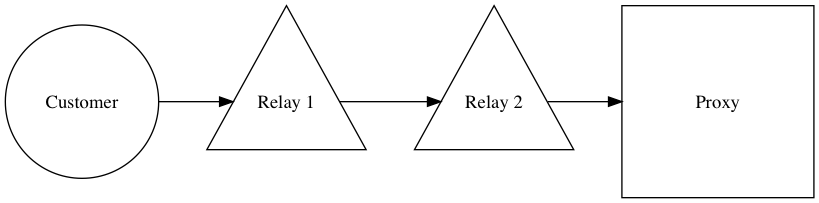
\includegraphics[width = 300pt]{sttc}
  \caption{A three-Econ Manifold routing traffic for a Customer}
\end{figure}

In this section we will describe the specification for Relay and Proxy
behavior, and discuss the ``chaining together'' of these nodes to
support uncensorable, anonymous web browsing.

\subsection{Specification for the Sale of Bandwidth}

Relay nodes implement a relatively simple behavior pattern:

\begin{itemize}
\item Maintain one or more connections, each with their own encryption key.
\item Check any tickets received, and cash-in winners.
\item Monitor the balance of trade, and disconnect if it exceeds a
  predeclared amount.
\item Receive data from any open connection, and perform decryption at
  message boundaries.
\item Process decrypted messages as follows:
  \begin{itemize}
  \item Forward any non-control segments to the connection(s)
    specified in the message.
  \item Process any control segments:
    \begin{itemize}
    \item \emph{Dummy Data.} Instructs the Relay to discard this segment.
    \item \emph{Burn at Rate.} Instructs the Relay to send data over a
      connection at a fixed rate, queueing packets and generating data
      as necessary to maintain the rate.
    \item \emph{Ratchet Ticket.} Instructs the Relay to pass a Ticket to
      the peer it received this packet from.
    \item \emph{Initiate Connection.} Instructs the Relay to establish a
      new connection. Used during setup and to handle disconnection.
    \item \emph{Initial Web Connection.} (Proxies Only.) Instructs the
      proxy to open an SSL connection to the specified host. To
      support whitelists, this cannot be a raw IP address.
    \end{itemize}
  \end{itemize}
\end{itemize}

%% [saurik: should we flesh out the above with packet specifics? I feel
%%   like *this* part of the document can/should be more specific than
%%   the rest, as we'd like transient nodes to be written more rapidly
%%   than full clients? Just a guess. - dls]

An important consideration in the above behavior is that no
proof-of-work is required of Relays on an ongoing basis. When combined
with all our connections being WebRTC connections, this leaves the
door open for websites potentially monetizing their visitors by
running pure javascript relay code.

For discussion of possible extensions via application specific control
segments, see Section \ref{sec:future}.

\subsection{Guard Nodes and ``Bandwidth Burning''}
\label{bandwidth-burning}

The relay that a customer is connected to has a very important piece
of information: the customer’s IP address. We assume customers will
want to keep this as private as possible, and so the default client
expresses a preference for long-lived peers as the first
hop.

Another concern for nodes at the first hop, which is discussed in
depth in our discussion of informational attacks stemming from
collusion (Section \ref{sec:collusion}), is they sit in an ideal
position to perform timing attacks. To prevent these attacks, we
recommend that privacy-conscious users employ a method called
\emph{Bandwidth Burning} -- paying the second hop to send a fixed
amount of bandwidth to the customer. As this approach results in
data-usage which is completely uncorrelated to network usage, this
approach prevents timing attacks performed by adversaries which cannot
see the inbound traffic of relay three.

To provide assistance to users seeking evasion (Section
\ref{sec:evasion}), bandwidth burning will also support non-fixed
rates determined by the statistical properties of popular non-Orchid
WebRTC protocols.

\section{Chaining and Informational Attacks on Manifolds}

The primary initial application of the above specification is the
creation of chains.

In this section we explore what kinds of information are available to different nodes for different manifold structures. Perhaps more importantly, we look at how different types of collusion change a user's privacy, and what the chance of such collusion are given $a$, the percentage of a network controlled by a given attacker, and $n$, the total size of the network.

\subsection{Information Available to a Relay or Proxy}
\label{relay-proxy-info-known}

Due to the inherent structure of IP-based networking, and the \mesh{} protocol, relay nodes gain access to the following information:

\begin{itemize}
\item The IP Addresses of both up and down. This is required to perform the IP communication.
\item The size, timing, and number of packets they forward. This is required if they are to forward packets.
\item A public Ethereum key owned by the user who is paying them. This is required for the selling of bandwidth.
\end{itemize}

\subsection{Collusion}
\label{sec:collusion}

Definition of Attacker roles:

\begin{itemize}
\item Global Adversary. An attacker with a global view of the network. Occurs with probability 1 in all cases.
\item ISP. The user's Internet service provider. Untrustworthy with probability $s$.
\item Web. The webserver the proxy is connected to. Untrustworthy with probability $w$.
\item Relay$_n$. The nth relay in the chain. Untrustworthy with probability $\frac{a}{n}$.
\item Proxy. The relay proxying bandwidth for the user. Untrustworthy with probability $\frac{a}{n}$.
\end{itemize}

Definition of attacks:

\begin{itemize}
\item Relation. When this is possible, the attacker can deduce the Customer of a Manifold simply by doing lookups of linked IP addresses.
\item Timing. By controlling the timing of packets a link which cannot be looked up can be inferred.
\end{itemize}

\subsection{Zero Relays, Zero Proxies: Direct Connection}

Although the \Mesh{} system is not used when a Customer connects directly to a website, we feel it is important to review what informational risk are present in this setup.

\begin{center}
\begin{tabular}{l | l | l | l | l | l}
  ISP & Website & P(Relate)          & P(Timing) \\
  \hline
  x   &         & $s$                & \\
  \hline
      & x       & $w$                & \\
\end{tabular}
\end{center}

\begin{itemize}
\item ISP can directly relate Customer traffic. $p = s$
\item Website alone can directly relate Website traffic. $p = w$
\end{itemize}

\subsection{Zero Relays, One Proxy}

\begin{figure}[htbp]
  \centering
  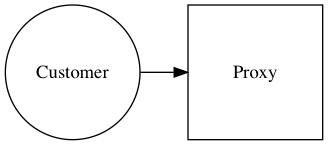
\includegraphics[width = 200pt]{sc}
  \caption{}
\end{figure}

\begin{center}
\begin{tabular}{l | l | l | l | l | l}
  ISP & Proxy & Website & P(Relate)          & P(Timing) \\
  \hline
      & x     &         & $\frac{a}{n}$      & \\
  \hline
  x   &       & x       &                    & $sw$ \\
\end{tabular}
\end{center}

\begin{itemize}
\item Proxy can relate Website traffic. $p = \frac{a}{n}$.
\item ISP + Website can relate Website traffic. $p = sw$.
\end{itemize}

\subsection{One Relay, One Proxy}

\begin{figure}[htbp]
  \centering
  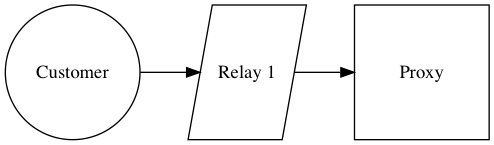
\includegraphics[width = 200pt]{stc}
  \caption{}
\end{figure}

\begin{center}
\begin{tabular}{l | l | l | l | l | l}
  ISP & Relay$_1$ & Proxy & Website & P(Relate)          & P(Timing) \\
  \hline
      & x         & x     &         & $(\frac{a}{n})^2$  & \\
  \hline
      & x         &       & x       & $w(\frac{a}{n})$   & \\
  \hline
  x   &           & x     &         & $s(\frac{a}{n})$   & \\
  \hline
  x   &           &       & x       &                    & $sw$ \\
\end{tabular}
\end{center}

In the one Relay one Proxy case.


\begin{itemize}
\item Relay$_1$ + Proxy can relate customer traffic. $p = (\frac{a}{n})^2$
\item Relay$_1$ + Website can relate Website traffic. $p = w\frac{a}{n}$
\item ISP + Proxy can relate all Website traffic. $p = s\frac{a}{n}$
\item ISP + Website can timing attack Website traffic. $p = sw$
\end{itemize}

\subsection{Two Relays, One Proxy}

\begin{figure}[htbp]
  \centering
  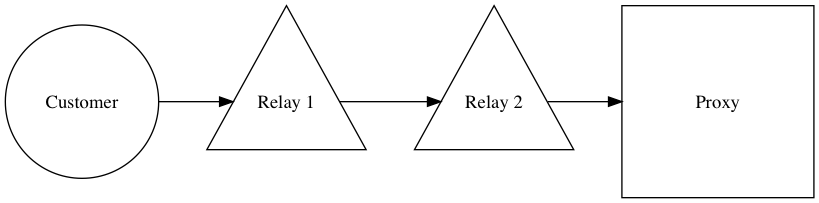
\includegraphics[width = 200pt]{sttc}
  \caption{}
\end{figure}

\begin{center}
\begin{tabular}{l | l | l | l | l | l | l}
%\begin{tabular}{l*{7}{c}r}
  ISP & Relay$_1$ & Relay$_2$ & Proxy & Website & Relate             & Timing \\
  \hline
      & x         &           & x     &         & $(\frac{a}{n})^2$  & \\
  \hline
  x   &           & x         & x     &         & $s(\frac{a}{n})^2$ & \\
  \hline
      & x         & x         &       & x       & $w(\frac{a}{n})^2$ & \\
  \hline
  x   &           & x         &       & x       & $sw(\frac{a}{n})$  & \\
  \hline
      & x         &           &       & x       &                    & $s(\frac{a}{n})$ \\
  \hline
  x   &           &           &       & x       &                    & $sw$ \\
\end{tabular}
\end{center}

In the more familiar two Relays one Proxy case, we can see now.

\begin{itemize}
\item Proxy + Relay$_1$ can relate customer traffic. $p = (\frac{a}{n})^2$
\item Proxy + Relay$_2$ + ISP can relate customer traffic. $p = s(\frac{a}{n})^2$
\item Website + Relay$_1$ + Relay$_2$ can relate Website traffic. $p = w(\frac{a}{n})^2$
\item Website + Relay$_2$ + ISP can relate Website traffic. $p = sw\frac{a}{n}$
\item Website + Relay$_1$ can timing attack Website traffic. $p = w\frac{a}{n}$ [can be prevented with bandwidth burning]
\item Website + ISP can timing attack Website traffic. $p = sw$ [can be prevented with bandwidth burning]
\end{itemize}

Total risk without bandwidth burning is therefore: $$(1+w+s)(\frac{a}{n})^2 + (sw+w)\frac{a}{n}$$ and $$(1 + w + s) (\frac{a}{n})^2$$ with bandwidth burning.

\subsection{Three Relays, One Proxy}

\begin{figure}[htbp]
  \centering
  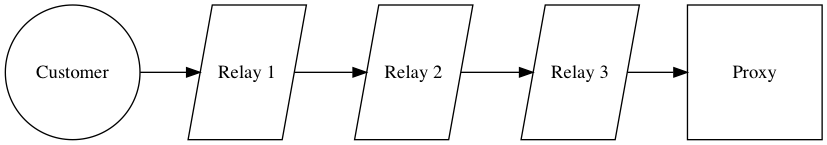
\includegraphics[width = 200pt]{stttc}
  \caption{}
\end{figure}

\begin{itemize}
\item Proxy + Relay$_1$ + Relay$_2$ can relate customer traffic. $p = (\frac{a}{n})^3$
\item Proxy + Relay$_1$ + Relay$_3$ can relate customer traffic. $p = (\frac{a}{n})^3$
\item Proxy + Relay$_2$ + ISP can relate customer traffic. $p = s(\frac{a}{n})^2$
\item Website + Relay$_1$ + Relay$_3$ can relate Website traffic. $p = w(\frac{a}{n})^2$
\item Website + Relay$_2$ + Relay$_3$ + ISP can relate Website traffic. $p = sw(\frac{a}{n})^2$
\item Website + Relay$_1$ can timing attack Website traffic. $p = w\frac{a}{n}$ [can be prevented with bandwidth burning]
\item Website + ISP can timing attack Website traffic. $p = sw$ [can be prevented with bandwidth burning]
\end{itemize}


\section{SSL and TLS Vulnerabilities}

SSL Downgrade

\subsection{The old browser problem}

\subsection{The old phone app problem}

\subsection{Mitigation of 8.1.1 and 8.1.2}

\begin{enumerate}
\item Check SSL Certificates
\item Check SSL Versions, Cipher Suites
\item Check Basic Constraints
\item “Boring SSL”
\end{enumerate}


\section{The Agora}
\label{sec:agora}

The Agora, named after the greek work for market, is a P2P network
similar in structure to a Distributed Hash Table (DHT), which serves
as a meeting ground for buyers and sellers of bandwidth.

\subsection{Fundamental Agora Operations}

At a high-level, the operations provided by the Agora are:

\begin{itemize}
\item A method for Econs to join the Agora.
\item A method for asking Econs what services they have for sale.
\item A method for selecting a subset of all peers, randomly weighted by computational resources, such that the \emph{lookup property} holds: $$lookup(rand(address)) \approx rand(Econ)$$
\end{itemize}

The \emph{lookup property} is important because it allows customers to
know with assurance that their chosen Econ is an attacker with
probability $\frac{a}{n}$.

To implement these operations, the Agora takes the structure of a DHT
with no keys and values. To perform the random selection, a user
simply generates a random address and locates the Econ closest to that
point.

\subsection{Fundamental Econ Operations}

The operations supported by Econs on the Agora are:

\begin{itemize}
\item \emph{Get Routing Table and Medallion}. This returns the Econ's proof of work and signed routing table for inspection, along with the cost of relaying traffic to members of the routing table.
\item \emph{Relay Traffic}. Pays the Econ to forward traffic to one of the peers in its routing table.
\item \emph{List Services}. Asks the Econ for a list of services it sells.
\item \emph{Purchase Service}. Employ the Econ as a service provider.
\end{itemize}

The first two of these are used by customers to navigate to an Econ of
interest, while the second two are used to negotiate the purchase of
services once that Econ is found.

Navigation through the Agora takes a form similar to that used in
Manifolds. A customer connects to some known Econ (found through
bootstrapping, see \ref{bootstrapping}), inspects its routing table,
and pays to forward traffic to the Econ closest to its chosen
point. As we will see in the section on routing tables, this allows
customers to keep their IP addresses secret, while still providing
relatively efficient random access to Econs of $O(log^2 n)$ packets.

\subsection{Chord Routing Structure}

[need graphic]

Econs are connected in the \mesh{} Protocol using the same scheme used
in the Chord DHT.

Addresses are viewed as a ring of size $2^{256}$, and the distance
between peers at addresses $a, b \in [0, 2^{256}-1]$ is defined to be
$n$ s.t. $0 \leq n < 2^{256}$ and $a + n \equiv b \pmod{2^{256}}$.

For a collection of Econs in an Agora, $A$, the forced connections for
a given Econ $e$ are defined to be $\min_{f \in A} dist(e+t, f)$, for
each of 256 target addresses $t \in \{1, 2, 4, .. 2^{255}\}$.

We chose to use this routing structure because of its maturity,
successful track record in deployed systems, and correctness
proofs. Readers interested in learning more are encouraged to read
\ref{}. For our purposes, it is enough to note that the following two
properties are provided by this routing scheme:

\begin{enumerate}
\item \emph{Finite, Deterministic Connections}. Every Econ has a
  number of forced connections $\leq 256$.
\item \emph{Logarithmic Traversal Distance}. Given a random address
  $t$ and a random connected Econ $e$ with connections $C$, that
  $distance(e, t) \approx 2 * \min_{f \in C} distance(f, t)$. Because
  the distance will half with each hop, the expected traversal length
  on the network is $log_2(n)$ where $n$ is the network size.
\end{enumerate}

\subsection{Medallions on the Agora}

To prevent attackers from choosing their location on the Agora, the
location of Econs is defined to be the hash of their Medallion.  To
prevent an attacker from running more Econs than is proportional to
their share of the Agora's total computational power, every Econ
checks the validity of all its connections' Medallions every Medallion
cycle. In the event that a valid Medallion is not supplied, it is
disconnected from the network.

\subsection{Signed Routing and Eclipse Attacks}

%% In a fully distributed system, no one (except, perhaps, an attacker)
%% has a global view of the network. Attackers often seek to exploit this
%% by choosing to omit mention of options they do not wish others to use.

%% For example, imagine if in the above routing scheme an attacker chose
%% to lie about what connections it has – if the buyer has no way of
%% detecting this, they might be led off to a fake Agora in which all
%% ``participants'' were owned by the attacker. To put a stop to this
%% situation, Agora's routing tables are verified non-malicious by the
%% peers contained on them via an inductive proof.

%% To do this, an Econ joining the network first computes its forced
%% connections list $C$, then demonstrates to each $c \in C$ that (1)
%% every connection in $C$ is indeed forced, and (2) it is possible to
%% route from every element of $C$ to every other element. It does this
%% by supplying the chain of signed routing tables that led it to each
%% element of $C$.

%% Once the proof has been sent




%% When a node would like to establish a forced connection, that node
%% must first prove to each node on its forced connections list that each
%% other node on that list is a member of the same Agora. To do this, we
%% show them a chain of routing tables that connects them.


One of the issues that arises in distributed networks is that no one (except, perhaps, an attacker) has a global view of the network. For example, imagine if in the above routing scheme an attacker chose to lie about what connections it has – if the buyer has no way of detecting this, they might be led off to a fake Agora in which all “participants” were owned by the attacker. To put a stop to this situation, Agora's routing tables are verified non-malicious by the peers contained on them.

When a node would like to establish a forced connection, that node must prove to each node on its forced connections list that each other node on that list is a member of the same Agora. To do this, we first select a random econ $G$ by finding the Econ with an address closest to the hash of all the connections in the routing table $H(C_i)$. Then we supply:

\begin{enumerate}
\item Proof that all the Econs on the list can all route to $G$.
\item Proof that $G$ can route to each Econ
\item Proof that each Econ on the list is indeed a forced connection.
\end{enumerate}

These proofs all take the form of signed routing table chains which lead from $C_i$ to $G$, or in the case of (3) the chain of signed routing tables which led from the Entry Econ to each $C_i$. Once such proof has been provided, all of the peers on the new routing table sign the table, and the connecting Econ signs theirs. For those elements of $C_i$ for whom the new Econ is a forced connection, the same proof is sent to each of their connections for signature.

Because this is the only method for adding Econs to the Agora, these requirements form an inductive proof of the Agora's soundness. If one of the nodes in $C_i$ attempts to supply a fake routing table, it will not route to the same $G$ as the other Econs in $C_i$. If one of the nodes $C_i$ is not a member of the Agora, $G$ will not be able to route to them. If the Econ seeking to connect has lied about $C_i$ being nearest nodes to his forced connection points, (3) will demonstrate that to be false.

From these properties, we can see that the avenues left for an attacker are:

\begin{itemize}
\item If an attacker can generate a Medallion address such that all $C_i$ are controlled by them, the above system will cease to function. This will happen with probability $(\frac{a}{n})^{log(n)}$. If such a collision occurs, $(1 - \frac{n-log(n)}{n})^{log(n)}$ percent of all queries will be compromised. To put these numbers in perspective, if an attacker controls 10\% of the network, at 1 million nodes there is a 1e-8\% chance of such a collision happening, and if it does occur around 1e3\% of all system queries will be impacted. At 100 million nodes the chance drops to 1e-12\%, causing disruption of 1e-5\% of queries. Note this damage is repaired during Agora Regeneration \ref{agora-regen}.
\item If an attacker has now joined the network, but was forced to use a valid routing table, the only attacks it can perform are related to selling services, not routing traffic on the Agora. As this is the situation expected in the rest of our attack models (that an attacker will control a number of econs proportional to the computational resources), we do not consider this an attack.
\end{itemize}

\subsection{Eclipse Attacks and Regeneration}
\label{agora-regen}

Long lived P2P networks suffer from Eclipse attacks. Although the
above signed routing scheme can make these arbitrarily difficult by
involving ever increasing number of peers for verification, another
approach is simply to limit the lifespan of peers. For this reason,
Econs on the Agora must change keys every 100 Ethereum blocks.

This is ensured by $XOR(address, Eth)$

[Todo: finalize randomization schedule here.]

\subsection{Finding Entry Nodes}
\label{bootstrapping}

The distribution of Entry Nodes is a difficult topic. If oppressive governments are able to access this list, they will block user's abilities to access the list. We have therefore located essential services that would be internet-breaking if they were blocked, and have devised methods for adding Entry Node information to the data contained in them.

\subsection{Identifying \emph{the} Agora}

The above discussion discussion of security is ultimately meaningless if there is no way to locate ``the right Agora'' on a fresh machine. Any distribution method which exists for \emph{Entry Econs} can not be presumed immune from infiltration by fake Entry Nodes. To do so, we simply estimate the computing power of a given Agora, and select the right one. This is justified by our core security assumptions (Section \ref{core-security}).

\begin{itemize}
\item Density Estimation. Because an Econ's forced connections are defined to be the econs nearest to some set of points in a $2^{256}$ address space, in any real-world situation there will be measurable gaps between the ideal connections and the actual ones. To estimate density in this space, we can observe that these connections as the result of a random binomial process: every point between the ideal point and the actual point is a failure, and the actual point is a success. Therefore, for a given number of missing nodes $M$ and a given number of realized connections $C$, The uniform prior MAP estimate of network density is $$\frac{C}{C + M} 2^{256}$$.
\item Traversal Distance. The Agora provides address look ups in $O(log_2(n))$ hops. We can use this in reverse to estimate network density.
\end{itemize}

One might be inclined to believe that density estimation is enough, however a clever attacker in possession of a sybil network of modest size, will have free choice for which node is to be put forward as the the Entry Econs for the false network, while the Entry Econs from the ``real Agora'' will have a density which is a random sample from the network. To make matters worse, if the traversal distance is chosen as the metric, one might imagine an attacker who anticipates this, and so creates sub-optimal routing tables which require longer than the $O(log_2(n))$ to traverse. Thankfully, sub-optimally connected Agoras will perform worse on the density metric. The verification method used in the \mesh{} System is to traverse to a random address, saving the routing tables along the way, and then perform a density estimate using the routing table from all but the first two hops.

%% \subsection{Economics}

%% \subsubsection{Price Discovery}

%% Uers may set their own price for bandwidth, but this is hardly
%% satisfying. Some users may price themselves out of the market, and
%% other users may charge too little. We therefore provide the following
%% algorithm for users who wish to maximize their profit as bandwidth
%% sellers:

%% \begin{algorithm}[H]
%%   \KwData{Quantity of bandwidth the user wishes to sell, $Q$}
%%   \KwData{Amount of data sold in the last 10 minutes, $S_t$}
%%   \KwData{Price of the previous data sold, $P_t$}
%%   \KwResult{A New Price $P_{t+1}$}
%%   \While{$S_t > Q$}{
%%     return $S_t$ * 1.1;
%%   }
%%   return $(S_t - Q) * 0.01 * P_t$ ;
%%   \caption{Automatic Price Scaling}
%% \end{algorithm}

%% \subsubsection{Auction Design}

\subsection{Proxy Whitelists}

Some users wishing to offer Proxy services may not be comfortable offering ``open access''. For example, allowing users to access facebook.com has a risk profile similar to acting as a relay, while allowing arbitrary connections to the internet may result in a visit from local law enforcement. Econs on the Agora may therefore set a whilelist of websites they will allow users to contact when using them as a Proxy, and specify their whitelists in their responses to \emph{Get Offers}.

%% \subsection{Informational Attacks}

%% \subsubsection{Learning All Econ IP Addresses}

%% The number of forced connections grows at roughly $log_4(N)$ where N
%% is the network size. If an attacker holds $m\%$ of global computation,
%% they will be able to create $c = 10mlog_4(N)$ connections ip addresses
%% per key rotation. The expected number of IP addresses seen by the
%% attacker is then, $seen_t = (1-\frac{seen_t}{N})c$


\section{Economic Soundness}
\label{sec:economic-soundness}

.

\section{Firewall Circumvention Features}
\label{sec:evasion}

The above system would be of little use if only users already
possessing free and open access to the Internet could use it. In this
section we will discuss features which ease access for those users
whose Internet access is provided by their attacker.

Please note that if an adversary is willing to completely block all
Internet access, no defense in this area is possible. All defense
analysis in this section therefore assumes that the attacker suffers
some cost for blanket blocking, and seeks to maximize this cost in the
hope that sufficiently costly attacks will not be performed.

\subsection{Bootstrapping}

One of the first attacks we anticipate firewall providers to attempt
against the Orchid Network is to create a list of Entry Econs, and to
block all access to them. This is because if customers can not access
Entry Econs, they could not use the network. Complicating matters, a
competent attacker must be assumed to have any list of IP addresses
available to customers.

To address this initially, we will provide a service which allows
users to perform a ``group buy'' of a small VPS instance to act as a
relay in exchange for tokens. Customers would then use this relay as a
mechanism for accessing the rest of the network, making the security
analysis identical to that in Section \ref{sec:collision}, with Orchid
Labs also acting as a secondary ISP. Since this VPS's IP address is
drawn from IP addresses used to host websites generally, we anticipate
that blanket blocking of these IP addresses would be quite costly.

To hinder blocking of the bootstrapping back and forth itself, we will
provide access to this boostrapping service via web, email, and
popular instant messaging platforms. The user will copy/paste a
challenge from their client's options screen into the most convenient
communications mechanism, then copy/paste the reply back into the
client.

\subsection{Deep Packet Inspection, Timing Inference, and Active Probing of Connections}

More sophisticated firewalls employ methods such as deep packet
inspection (analysis of the contents of packets rather than just the
headers), timing inference (the use of aggregate statistical measures
over packet size, quantity, and timing), as well as active probing
(attempting connection with the user or the server they are connecting
to in an attempt to identify the service being provided.)

We do not anticipate the use of deep packet inspection or active
probing to provide significant information. Through our use of WebRTC,
all communication is encrypted and there are no open ports unless an
active WebRTC offer has been issued. Since this matches the behavior
of all other uses of WebRTC, this behavior can not disambiguate Orchid
users.

Timing inference is potentially an effective method for detecting
Orchid users, as the timing and size of web requests over an encrypted
stream are unlikely to look like other kinds of WebRTC traffic
(\cite{peekaboo}). To address this, users accessing the Orchid Network
in situations where inference attacks are likely are encouraged to use
``bandwidth burning'' (Section \ref{bandwidth-burning}).

\subsection{Disclosure: Ethereum Traffic}

Because the current client employs an Ethereum client to track payment
statuses, and Ethereum has its own non-hardened networking signature,
detection related to this Ethereum traffic is likely to be the weak
link. Firewall operators may simply ask ``is the computer running
Ethereum \emph{and} consuming large amounts of WebRTC traffic?''

To maintain project focus, hardening of Ethereum and/or serving
Ethereum traffic over the Orchid Network is not a feature of our
initial release. We plan on addressing this in future versions.

\section{Current State of the Software}
\label{sec:current}

[Note the current state of the software is: being actively coded right
now. The following describes where we will be at the time of
whitepaper release.]

\section{Performance Scaling}
\label{sec:performance}


\section{Attack Analysis and Attacker User Stories}
\label{sec:attack-stories}

\subsection{Oppressive Web Applications}

Attacker Goals: Identify all \Mesh{} Proxy IP addresses.

\subsection{Corporate Networks}

Attacker Goals: Prevent usage of the \Mesh{} network.

Resources: The attacker controls the network, and so can engage in traffic shaping and connection dropping.

\subsection{Passive Monitoring and Inference, perhaps with Sybil Attacks}

Attacker Goals: Learn Customer IP Identification, and Website Identification.

Resources: An attacker has view of some amount of passive network surveillance, and is able to add nodes to the network up to $s\%$ as a source of additional data.

\subsection{Great Firewalls}

Attacker Goals: Prevent usage of the \Mesh{} network.

Resources: The attacker controls the network, has passive surveillance of it, and is able to add nodes up to $s\%$ of the network size.

\subsection{Small-Time Mayhem and QoS Attacks}

Synopsis: An attacker would like to cause mayhem on as much of the network as possible.

Resources: On the order of ten thousand dollars of networking and computation ability.

% \subsection{Exploitative End Users (Vigna)} -- I think they might have the same ``goals'' as all other attackers, or else it's not really security research.


\section{Future Work}
\label{sec:future}

The items in this section fall into two categories: nice-to-haves, and features we are internally conflicted about releasing to the public. We believe this is conflictedness is universal -- although almost everyone has favorite examples of power being used for oppression, there are also countless examples of power being used for good. Protocols like \Mesh{} have no judgement of their own, and so cannot tell if they are routing traffic for a freedom fighter or a terrorist, villain or hero.

\subsection{Proof of Space}
\label{future:proof-of-space}

Exploding function, way of verifying.

\subsection{Content Storage}
\label{subsec:ccn}

The issue with modern networking from an surveillance perspective is that it is fundamentally about connections between computers. So long as the model is that a user's computer connects to a specific webserver to access a website, \Mesh{} may be as good as possible. However, if we

\subsection{Saturated Links}
\label{subsec:saturated-links}

TODO: this would have to be the standard global protocol to work. Idea is have every ``guard node'' send at 1MB/sec or so... Customers then pay for that bandwidth, rather than minimum amount of bandwidth needed (the regular case).

\subsection{Protecting Content Hosts}
\label{subsec:protocol-extentions}

Many prior approaches (Section \ref{sec:prior-approaches}) discovered that content hosts sought similar protections as web users. We are internally conflicted on this point, as we do believe there is content which it is in the public interest not to have freely distributed (information related to the manufacture of nuclear weapons for example). However, should unforseen circumstances demand it, \Mesh{} could be extended to support such ``unrestricted, unsurveilled Hosts'' as follows:

\begin{figure}[htbp]
  \centering
  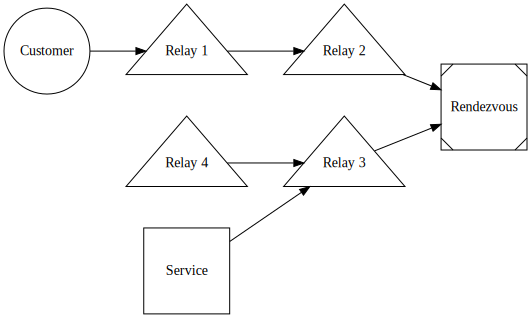
\includegraphics[width = 300pt]{sttRttc}
  \caption{A rendezvous node acting as a relay between a Service and a Customer}
\end{figure}

\subsection{Orchid as a Platform}

Although we anticipate that design of the core system will take up
much of our time for the immediate future, we are very interested in
the possibility that adding features to support the following use
cases may drastically increase the amount of bandwidth routed through
the Orchid Network.

\begin{enumerate}
\item APIs for websites to directly interface to the network, and
  incorporate tokens into their service.
\item Static Website Hosting and File Storage.
\item File Sharing.
\item (Okay, these require more build up I think:) an email/messaging
  service, arbitration services.
\end{enumerate}

\nocite{*}
\printbibliography

\end{document}
